\documentclass{report}
\usepackage{graphicx} % Required for inserting images
\usepackage[italian]{babel}
\usepackage{tikz}
\usepackage{hyperref}
\usepackage{amsmath}
\usepackage{xcolor}

\definecolor{darkgreen}{rgb}{0.0, 0.5, 0.0}


\title{Protezione e Integrità dei Dati nel Cloud}
\date{Parte V}

\begin{document}

\maketitle

\tableofcontents
\newpage

\chapter{Encryption}
Il \textit{server} potrebbe essere \textbf{\textit{honest-but-curious}}, non dovrebbe 
avere accesso alle risorse; voglio garantire confidenzialità anche rispetto a lui.

Un modo per ottenerla è utilizzare l'\textit{encyption}: si aggiunge 
un livello di protezione attorno ai dati sensibili che li rende non 
leggibili a chi non è autorizzato. 

Di base voglio avere una criptazione dei dati; il problema è il \textbf{bilanciamento tra protezione e funzionalità}, ovvero sulle \textit{query} che è possibile fare sui dati.

\subsubsection{Approcci per accesso a diversi livelli di granularità}

\begin{itemize}
    \item \textbf{\textit{Keyword-based searching:}} passo un \textit{token} già criptato 
    che viene usato per fare ricerca sui dati criptati (voglio trovare dove c'è una certa parola/espressione booleana)
    \begin{figure}[ht]
        \centering
        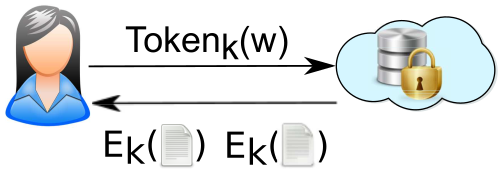
\includegraphics[width=0.4\linewidth]{images/encryption/token-based-search.png}
    \end{figure}
    \item \textbf{Crittografia omomorfica:} crittografia che supporta le operazioni direttamente sul cifrato
    \begin{figure}[ht]
        \centering
        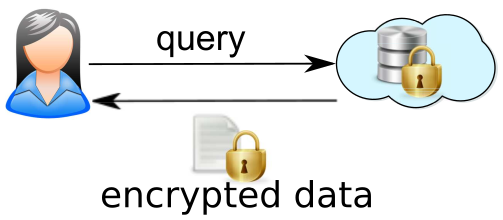
\includegraphics[width=0.4\linewidth]{images/encryption/homomorphic.png}
    \end{figure}
    \item \textbf{\textit{Encryption Schemas:}} ogni colonna può essere cifrata con un diverso schema crittografico 
    (\textit{random, add homomorphic, deterministic, order preserving, \dots})
    \begin{figure}[ht]
        \centering
        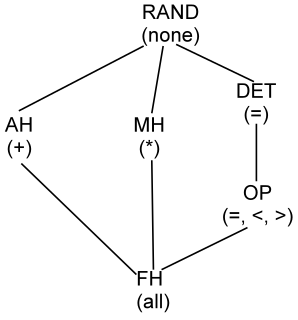
\includegraphics[width=0.3\linewidth]{images/encryption/schemas.png}
    \end{figure}
    \item \textbf{\textit{Onion Encryption:}} cifro i dati con diversi livelli \textit{a cipolla}, ognuno dei quali
    supporta l'esecuzione di una specifica \textit{query SQL}; l'idea è che \textit{scopro il dato solo quando mi serve}
    \begin{figure}[ht]
        \centering
        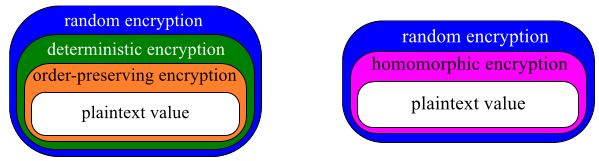
\includegraphics[width=0.8\linewidth]{images/encryption/onion.png}
    \end{figure}
    \item \textbf{Indicizzazione:} associo degli indici ai metadati
    \begin{figure}[ht]
        \centering
        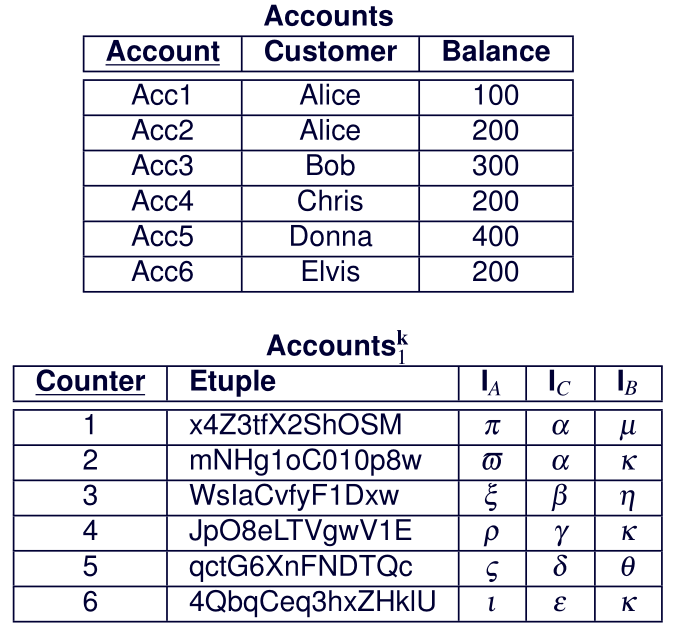
\includegraphics[width=0.6\linewidth]{images/encryption/indicizzazione.png}
    \end{figure}
    Nella seconda tabella: nella seconda colonna c'è la tupla criptata; nelle ultime tre ci sono gli attributi;
    si possono avere diversi tipi di indicizzazione:
    \begin{itemize}
        \item \textbf{\textit{Direct} $(1:1)$}
        
        \textcolor{darkgreen}{\textbf{+}} riesco a fare query precise
        
        \textcolor{red}{\textbf{-}} soggetto ad attacchi di frequenza
        \begin{figure}[ht]
            \centering
            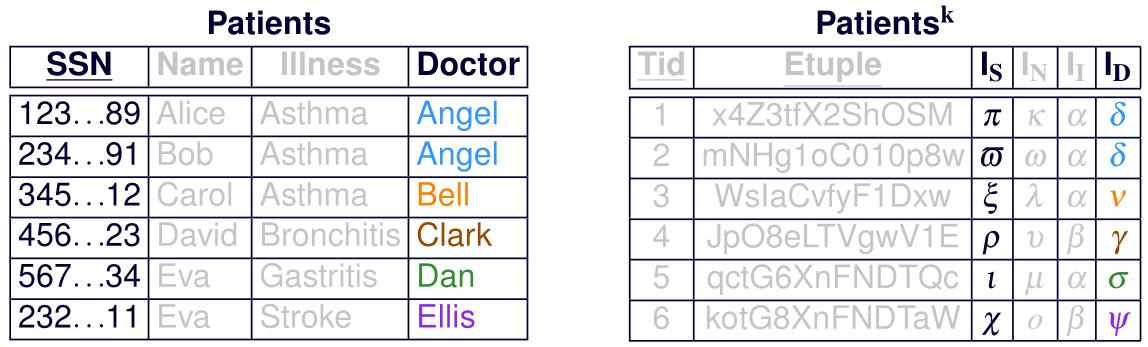
\includegraphics[width=0.85\linewidth]{images/encryption/index-direct.png}
        \end{figure}
        \item \textbf{\textit{Bucket} $(n:1) \rightarrow$} indicizzazione con collisione; ho diversi valori 
        che sono \textbf{mappati allo stesso indice}

        \textcolor{darkgreen}{\textbf{+}} non ho più attacchi di frequenze

        \textcolor{darkgreen}{\textbf{+}} supporta query di uguaglianza (\textit{se un valore è uguale ad un altro})
        
        \textcolor{red}{-} i risultati avranno delle tuple spurie

        \textcolor{red}{-} è ancora possibile fare qualche leakage
        \begin{figure}[ht]
            \centering
            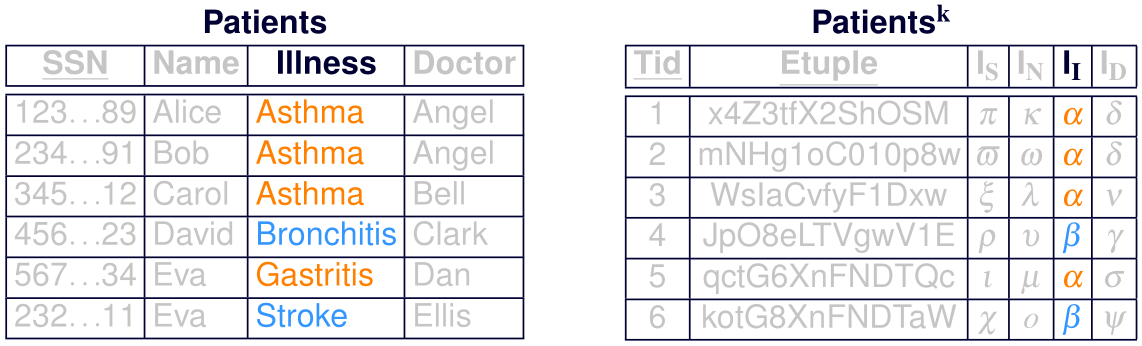
\includegraphics[width=0.85\linewidth]{images/encryption/bucket-index.png}
        \end{figure}
        \textit{In questo caso sono comunque esposto perché asma ha 3 occorrenze, dunque sarà per forza associata ad $\alpha$}

        \item \textbf{\textit{Flattened} $(1:n) \rightarrow$} ciascun indice deve avere lo stesso numero di occorrenze; significa che 
        i valori che hanno più occorrenze sono associati ad indici diversi

        \textcolor{darkgreen}{\textbf{+}} rimuovo la possibilità di fare attacchi di inferenze

        \textcolor{red}{\textbf{-}} sono esposto ad osservazioni dinamiche (magari certi dati sono sempre cercati assieme) 
        \begin{figure}[ht]
            \centering
            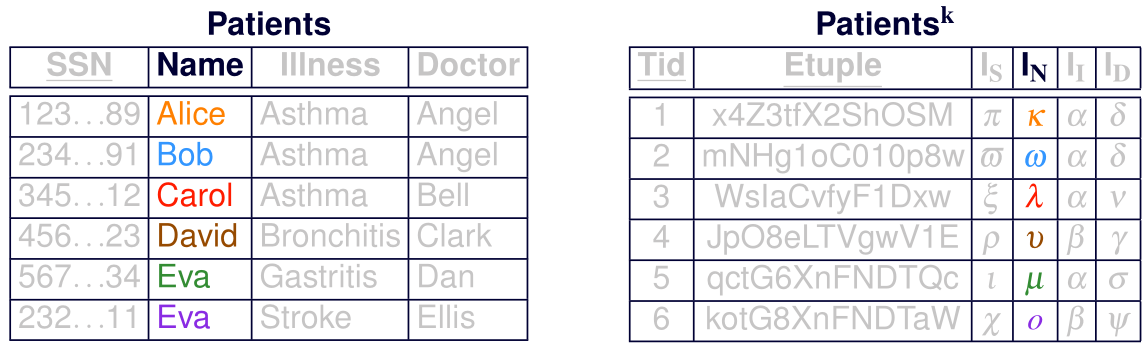
\includegraphics[width=0.85\linewidth]{images/encryption/flattened-index.png}
        \end{figure}

        \item \textbf{\textit{Partition-based:}}
        \begin{enumerate}
            \item si partiziona il dominio di un attributo
            \item a ciascuna partizione si assegna un'etichetta
            \item il valore in chiaro viene sostituito dall'etichetta
        \end{enumerate}

        \begin{figure}[ht]
            \centering
            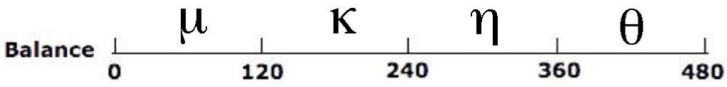
\includegraphics[width=0.6\linewidth]{images/encryption/partion-based-index.png}
        \end{figure}

        \noindent Supporta \textit{query} dove le condizioni sono espressioni booleane del tipo:

        - \textit{Attribute} \texttt{op} \textit{Value}

        - \textit{Attribute} \texttt{op} \textit{Attribute}

        dove \texttt{op}$=\{ =, <, >, \leq, \geq \}$

        \begin{figure}[ht]
            \centering
            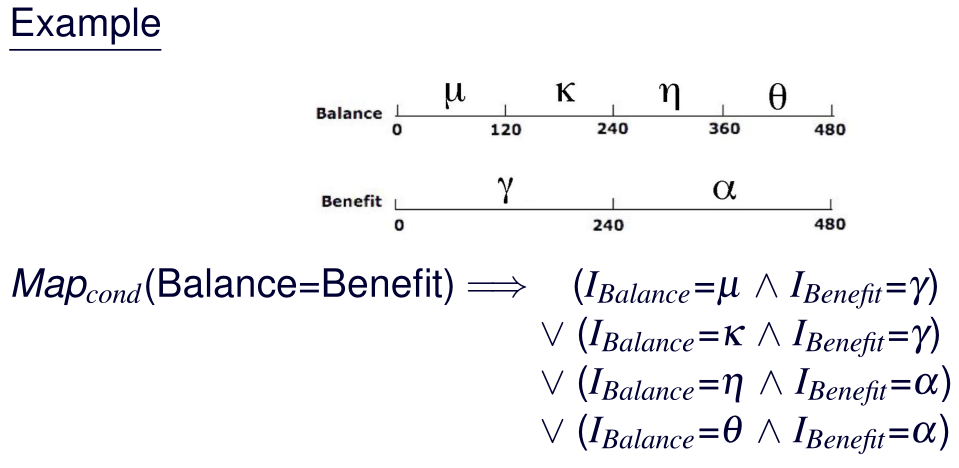
\includegraphics[width=0.6\linewidth]{images/encryption/partition-based-ex.png}
        \end{figure}

        \noindent \textbf{Esecuzione delle query:}

        \noindent Ogni query $Q$ sul DB in chiaro viene tradotta in:
        \begin{enumerate}
            \item una query $Q_s$ da eseguire sul server $\rightarrow$ query sull'indice per ottenere le tuple criptate
            \item una query $Q_c$ da eseguire sul client $\rightarrow$ decriptare il risultato della query precedente e filtrare le tuple spurie
        \end{enumerate}

        La traduzione dovrebbe essere fatta in modo tale che il server sia responsabile 
        della maggior parte del lavoro.

        \begin{figure}[ht]
            \centering
            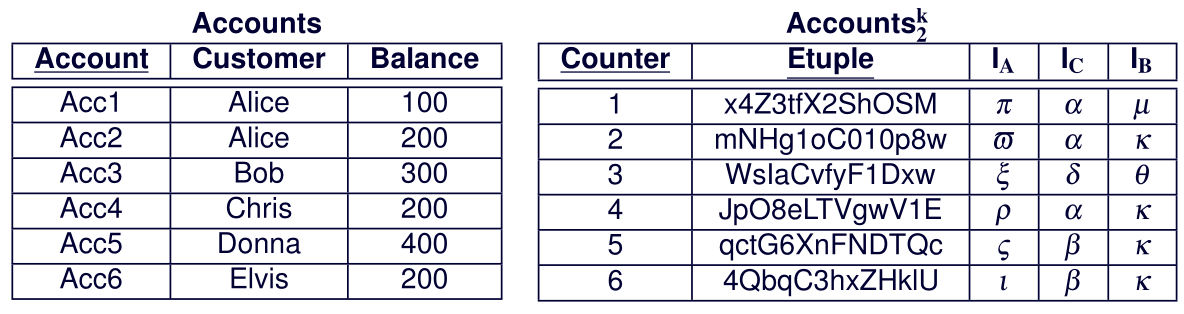
\includegraphics[width=0.8\linewidth]{images/encryption/query-ex-1.png}
        \end{figure}
        \begin{figure}[ht]
            \centering
            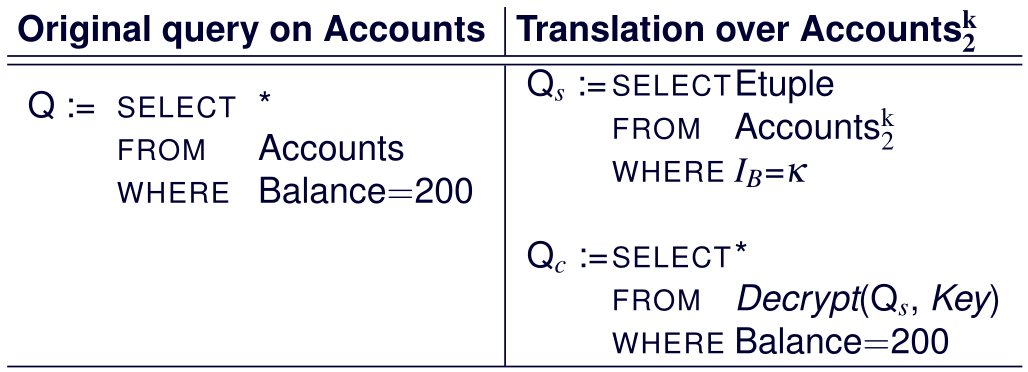
\includegraphics[width=0.8\linewidth]{images/encryption/query-ex-2.png}
        \end{figure}

        \newpage
        \item \textbf{\textit{Hash-based:}} basate sul concetto di \textit{one-way hash function}; ogni
        attributo viene mappato ad un indice utilizzando una funzione di hash sicura.

        \noindent Dat una funzione $h$ e il dominio degli attributi $D_i$, diciamo che $h$ è \textbf{sicura} se:
        \begin{enumerate}
            \item $\forall x, y \in D_i \implies h(x) = h(y)$ (\textbf{determinismo}) 
            \item dati due valori $x, y \in D_i$ tali che $ x \neq y$, potremmo avere che $h(x)=h(y)$ (\textbf{collisione}, per proteggermi da attacchi di frequenza)
            \item la distanza dei valori in chiaro deve essere \textbf{indipendente} dalla distanza dei valori di hash (\textit{strong mixing})
        \end{enumerate}

        \noindent Questo metodo supporta \textit{query} dove le condizioni sono espressioni booleane del tipo:
        \begin{itemize}
            \item $ Attribute = Value$
            \item $Attribute_1 = Attribute_2$, se sono indicizzati con la stessa funzione di hash
        \end{itemize}
        
        \noindent La traduzione funziona come nel metodo \textit{partion-based}; non 
        sono supportate \textit{query di range}. 
    \end{itemize}
\end{itemize}

\subsubsection{Interval-based queries}
\begin{itemize}
    \item Le tecniche di indicizzazione che preservano l'ordine supportano 
    query di range, ma sono esposte ad inferenza
    \item Le tecniche di incizzazione che \textit{non} preservano l'ordine non sono esposte 
    ad inferenza, ma non supportano query di range
\end{itemize}

$\rightarrow$ viene calcolato un $B_+ -tree$ dal client, ed ogni nodo viene criptato come un tutt'uno; successivamente 
per rispondere alle query l'albero viene visitato (in ambiente trusted).

\newpage
\section{\textit{Searchable Encryption}}
\subsection{\textit{Order preserving encryption}}
\begin{itemize}
    \item \textbf{\textit{Order Preserving Encryption Schema (OPES):}} prende in input una distribuzione target 
    di valori per gli indici ed applica una trasformazione che preserva l'ordine e rispecchia 
    la distribuzione di input.

    \textcolor{darkgreen}{\textbf{+}} la comparazione può essere fatta direttamente sui dati criptati 

    \textcolor{darkgreen}{\textbf{+}} le query non producono tuple spurie 

    \textcolor{red}{\textbf{-}} vulnerabile ad attacchi di inferenza

    \item \textbf{\textit{Order Preserving Encryption with Splitting and Scaling (OPESS):}}
    
    Questo schema crea degli indici in modo tale che la loro distribuzione delle frequenze sia piatta.
\end{itemize}

\subsection{\textit{Fully homomorphic encryption}}

\begin{itemize}
    \item Permette una performante computazione specifica sui dati criptati 
    \item Decriptando il risultato, si ottiene lo stesso risultato delle stesse operazioni sui dati in chiaro
\end{itemize}

\newpage
\section{Esposizione all'inferenza}

Ci sono due requisiti conflittuali quando si parla di 
\textit{indicizzare} dati:
\begin{itemize}
    \item gli indici dovrebbero fornire una \textbf{esecuzione delle query efficiente}
    \item gli indici non dovrebbero aprire porte ad attacchi di \textbf{inferenza} e \textit{linking}
\end{itemize}

$\rightarrow$ diventa importante misurare quantitativamente il livello di esposizione dovuto 
alla pubblicazione degli indici:

\centering $\epsilon =  $ \textit{Coefficiente di Esposizione}

\noindent La computazione del \textit{Coefficiente di Esposizione} dipende da diversi fattori:
\begin{itemize}
    \item \textbf{Metodo di incizzazione utilizzato}
    \begin{itemize}
        \item \textit{direct encryption}
        \item \textit{hashing}
    \end{itemize}
    \item \textbf{Conoscenza pregressa dell'attaccante}
    \begin{itemize}
        \item $Freq + DB^k$
        \item $DB + DB^k$
    \end{itemize}

    \noindent In entrambi i casi l'attaccante può risalire alla funzione di incizzazione.
\end{itemize}




\end{document}